\documentclass[a4paper,12pt]{article}
\usepackage[T1]{fontenc}
\usepackage[latin9]{inputenc}
\usepackage{listings}
\usepackage{amsmath}
\usepackage{mathtools}
\usepackage{hyperref}
\usepackage{mathpazo}
\usepackage{wasysym}
\usepackage{graphicx}
\usepackage[colorinlistoftodos]{todonotes}
\usepackage{natbib} 
\usepackage{geometry}
\usepackage{tikz}
\geometry{verbose,tmargin=2.5cm,bmargin=2.5cm,lmargin=3cm,rmargin=3cm}

\DeclarePairedDelimiter{\ceil}{\lceil}{\rceil}
\DeclarePairedDelimiter{\floor}{\lfloor}{\rfloor}
\newcommand{\ord}{\operatorname{ord}}

\newcommand*\circled[1]{\tikz[baseline=(char.base)]{
            \node[shape=circle,draw,inner sep=2pt] (char) {#1};}}

\begin{document}

\title{I/O-algorithms\\Project 3}

\author{Lasse Espeholt - 20093223\\
Kasper Nielsen - 20091182\\}

\maketitle

\pagebreak{}\tableofcontents{}\pagebreak{}

\section{Sorting}
In this exercise an I/O-efficient algorithm for removing duplicates in a multiset of $N$ elements is analyzed. As given in the hint in the exercise, the algorithm is based on merge-sort, where duplicates are removed as soon as they are found in the merge step.

The algorithm will be analyzed by giving an upper bound on the number of times an element is scanned during an execution of the algorithm. For illustration purposes consider Figure~\ref{fig:sorting:mergetree}. Since duplicates are removed as soon as they are found, no node in the merge tree can contain duplicates (the leaves are found by sorting the elements in internal memory and removing duplicates).

\begin{figure}[h!]
  \centering
  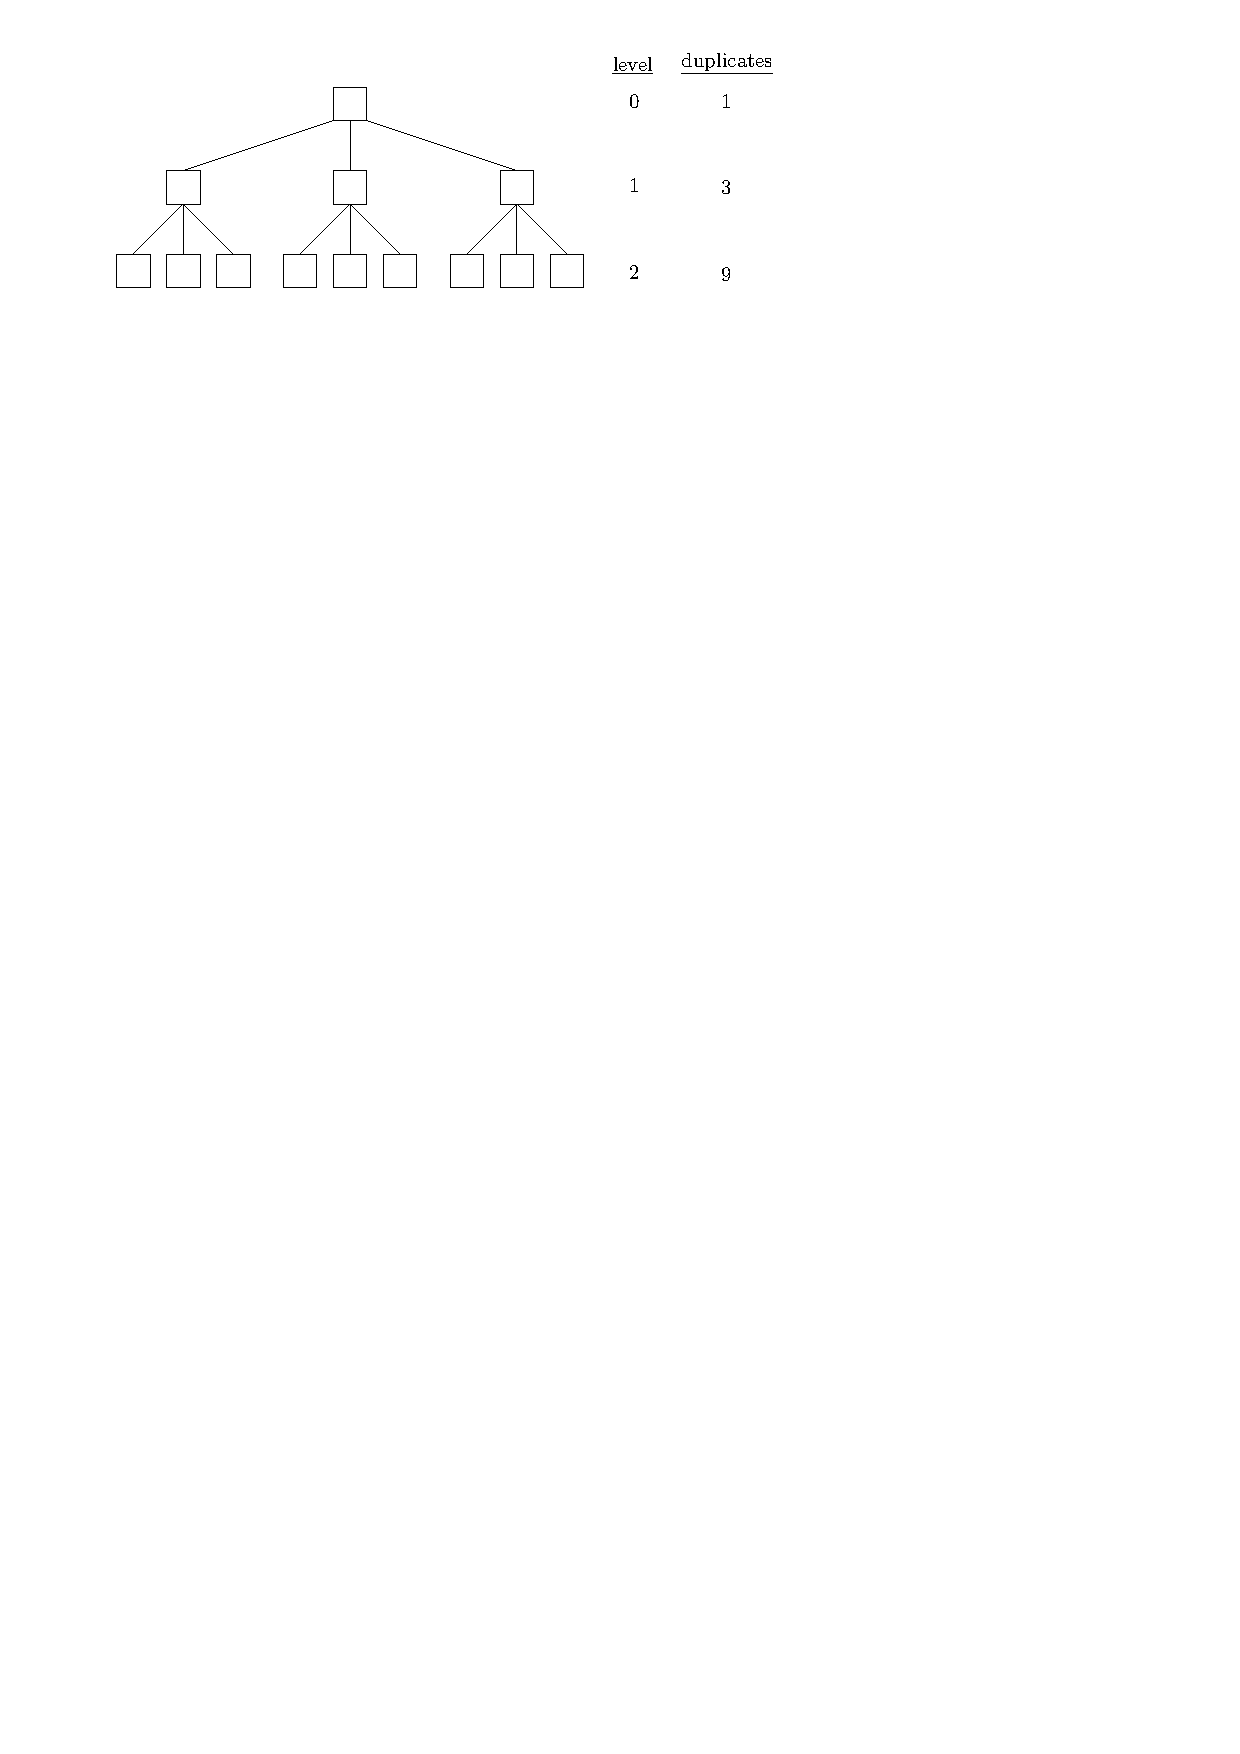
\includegraphics[width=0.8\textwidth]{images/mergetree}
  \caption{Example merge tree of height $3$ with fanout $d = 3$. Illustrates how many duplicates there can be on every level of the merge tree.}
  \label{fig:sorting:mergetree}
\end{figure}

Therefore for a given level $l$ in the merge tree of fanout $d$ and height $H$, at most $d^l$ duplicates remain. Furthermore, there is at most $N_i$ duplicates of a given element $i$. Therefore, the total number of duplicates remaining on level $i$ is less than $\min\{d^l, N_i\}$. Summing the contribution from all levels of the tree gives an upper bound on the number of times a given element is scanned. This can again be summed over all different elements, giving the following bound on the total number of element scans
\[
  \sum_{i=1}^K \sum_{l = 0}^H \min\{N_i, d^l\} .
\]
It is noticed that $N_i \leq d^l \iff \log_d{N_i} \leq l$. Therefore, if $H_i := \floor{\log_d{N_i}}$, then
\[
  \sum_{i=1}^K \sum_{l = 0}^H \min\{N_i, d^l\} =
    \sum_{i=1}^K \left( \sum_{l=0}^{H_i} d^l + \sum_{l = H_i + 1}^H N_i \right) =
    \underbrace{\sum_{i=1}^K \sum_{l=0}^{H_i} d^l}_{\circled{1}} + \underbrace{\sum_{i=1}^K \sum_{l = H_i + 1}^H N_i}_{\circled{2}}.
\]
An upper bound is given on \circled{1} and \circled{2}:
\begin{description}
\item[\circled{1}] Notice that\todo{Should we show this?}
  \begin{align*}
    \sum_{l=0}^{H_i} d^l = \frac{d^{H_i + 1} - 1}{d - 1} = \frac{d d^{\floor{\log_d{N_i}}} - 1}{d - 1} \leq \frac{d}{d - 1} N_i .
  \end{align*}
  When summing over all elements, it is found that
  \[
    \circled{1} \leq \sum_{i=1}^K \frac{d}{d - 1} N_i = \frac{d}{d - 1} N.
  \]
  By the tall cache assumption $d = \frac{M}{B} \geq B \geq 2$ (otherwise it is an internal memory algorithm). Therefore $\frac{d}{d - 1} \leq 2$, hence $\circled{1} = O(N)$.

\item[\circled{2}] For this bound, notice that
  \begin{align*}
    \sum_{l = H_i + 1}^{H} N_i &= \left( H - (H_i + 1) \right) N_i
      = \left( \log_d{\frac{N}{M}} - (\floor{\log_d{N_i}} + 1) \right) N_i \\
      &= \left( \log_d{\frac{N}{M}} - \log_d{N_i} \right) N_i
      = N_i \log_d{\frac{N}{M}} - N_i \log_d{N_i}.
  \end{align*}
  By summing over all elements, it is found that
  \[
    \circled{2} = \sum_{i=1}^K N_i \log_{\frac{M}{B}}{\frac{N}{M}} - N_i \log_{\frac{M}{B}}{N_i}
      = O\left( N \log_{\frac{M}{B}}{\frac{N}{B}} - \sum_{i = 1}^K N_i \log_{\frac{M}{B}}{N_i} \right).
  \]
\end{description}
Combining theses two bounds, it is found that at most
\[
  \sum_{i=1}^K \sum_{l = 0}^H \min\{N_i, d^l\} = O(N) + O\left( N \log_{\frac{M}{B}}{\frac{N}{B}} - \sum_{i = 1}^K N_i \log_{\frac{M}{B}}{N_i} \right)
\]
elements are scanned during the algorithm. The algorithm always scans elements in blocks, however some of the blocks could be non-full due to the duplicate removal. However, this can only happen once for every node in the merge tree, which is asymptotically bounded by the number of leaves ($\frac{N}{M} \leq \frac{N}{B}$). Therefore this cost and the cost of the first input scans are bounded by $O(\frac{N}{B}))$, whereby the total number of I/Os is bounded by
\begin{align*}
  O\left( \max\left\{ \frac{N}{B}, \frac{N \log_{\frac{M}{B}}{\frac{N}{B}} - \sum_{i = 1}^K N_i \log_{\frac{M}{B}}{N_i}}{B} \right\} \right) \\
    = O\left( \max\left\{ \frac{N}{B}, \frac{N}{B} \log_{\frac{M}{B}}{\frac{N}{B}} - \sum_{i=1}^K \frac{N_i}{B} \log_{\frac{M}{B}}{N_i} \right\} \right).
\end{align*}

\section{Searching}

...

\section{Distribution sweeping}

...

%\bibliographystyle{plain}
%\addcontentsline{toc}{section}{\refname}\bibliography{ref}

\end{document}
